\begin{frame}[allowframebreaks]{Contrastive Predictive Coding (CPC)}
    \begin{figure}
        \centering
        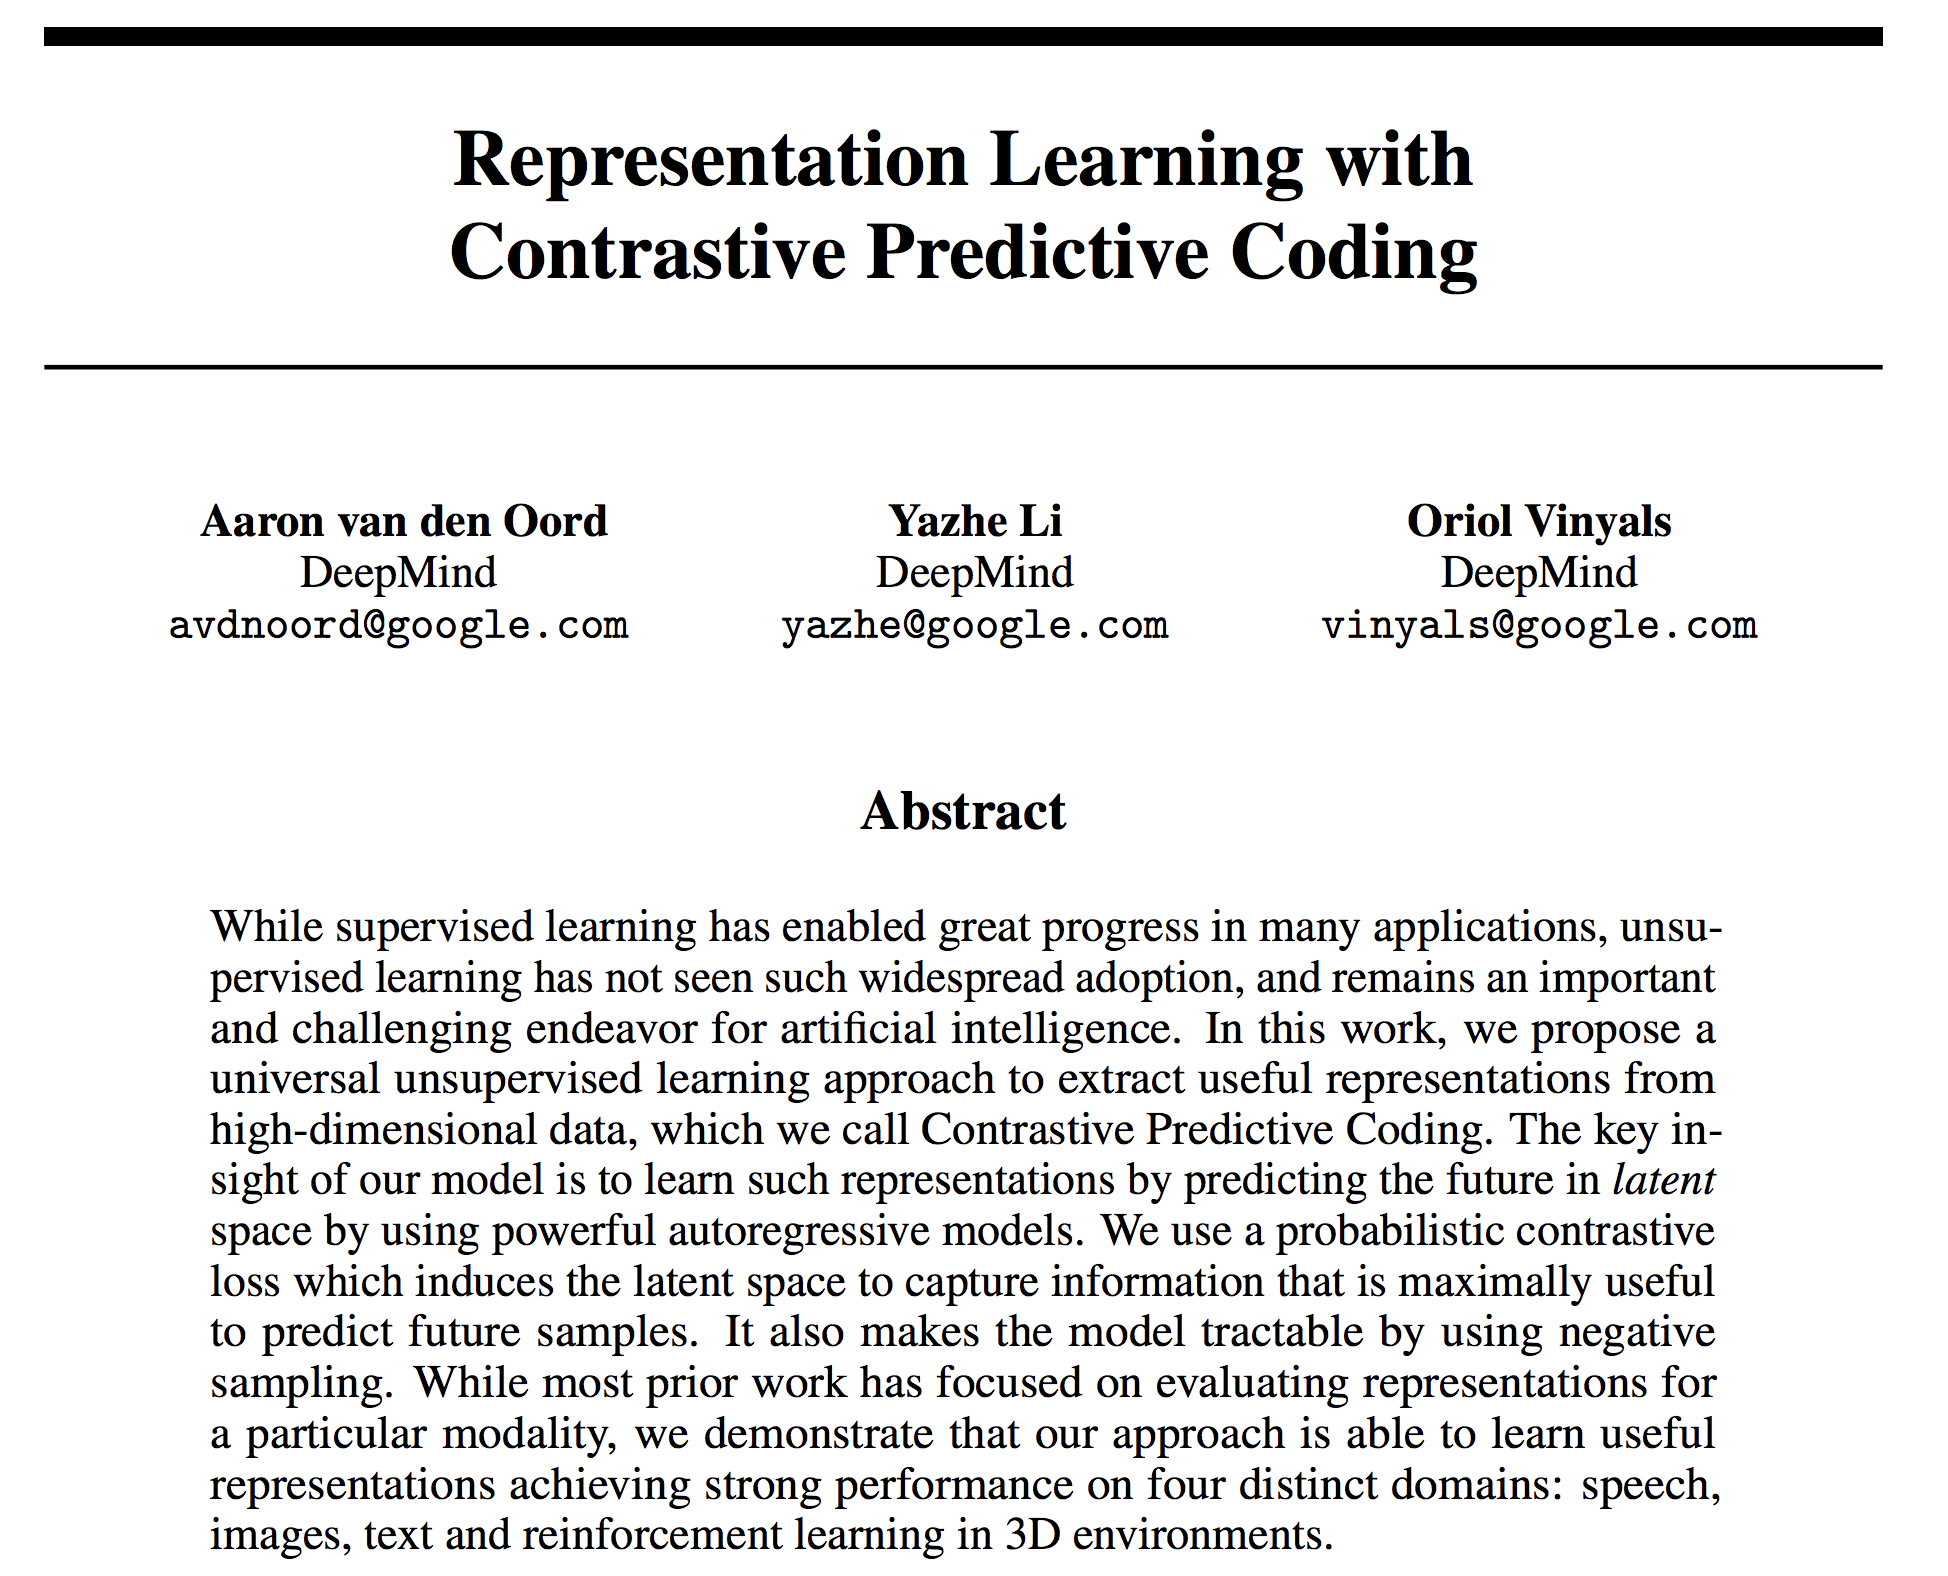
\includegraphics[width=1\linewidth,height=0.9\textheight,keepaspectratio]{images/ssl/slide_44_1_img.png}
    \end{figure}

    \framebreak

    \textbf{Contrastive Predictive Coding (CPC)} learns useful representations by predicting future information in latent space using powerful autoregressive models. The key components of CPC are:

    \begin{itemize}
        \item \textbf{Encoder}: Maps the input sequence $\mathbf{x}_t$ to a sequence of latent representations $\mathbf{z}_t$.
        \begin{itemize}
            \item Typically implemented as a convolutional or recurrent neural network.
            \item $\mathbf{z}_t = \text{Encoder}(\mathbf{x}_t)$
        \end{itemize}
        \item \textbf{Autoregressor}: Aggregates the sequence of past latents $\{\mathbf{z}_1, \ldots, \mathbf{z}_t\}$ into a context vector $\mathbf{c}_t$.
        \begin{itemize}
            \item Often implemented as an RNN or masked transformer.
            \item $\mathbf{c}_t = \text{AR}(\mathbf{z}_{\leq t})$
        \end{itemize}
        \item \textbf{Prediction}: The model predicts future latent representations using the context vector.
        \begin{itemize}
            \item For each step $k$, a linear transformation $W_k$ is applied to the context: $\hat{\mathbf{z}}_{t+k} = W_k \mathbf{c}_t$
            \item The goal is to distinguish the true future latent $\mathbf{z}_{t+k}$ from negative samples.
        \end{itemize}
        \item \textbf{InfoNCE Loss}: A contrastive loss that encourages the predicted future latent to be similar to the true future latent and dissimilar to negative samples.
        \begin{itemize}
            \item For each prediction step $k$:
            \[
                \mathcal{L}_{\text{InfoNCE}} = -\mathbb{E} \left[ \log \frac{\exp(\mathbf{z}_{t+k}^\top W_k \mathbf{c}_t)}{\sum\limits_{j} \exp(\mathbf{z}_j^\top W_k \mathbf{c}_t)} \right]
            \]
            \item The denominator sums over one positive and multiple negative samples.
        \end{itemize}
    \end{itemize}

    \framebreak

    \begin{figure}
        \centering
        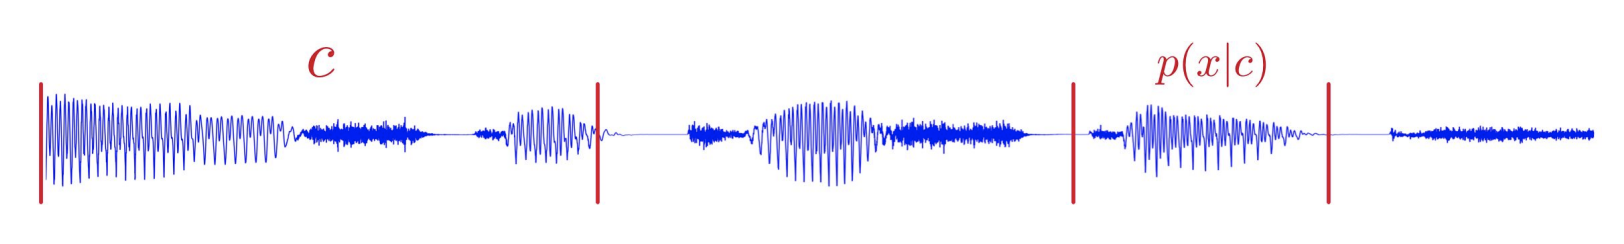
\includegraphics[width=1\linewidth,height=0.9\textheight,keepaspectratio]{images/ssl/slide_45_1_img.png}
    \end{figure}

    \framebreak

    \begin{figure}
        \centering
        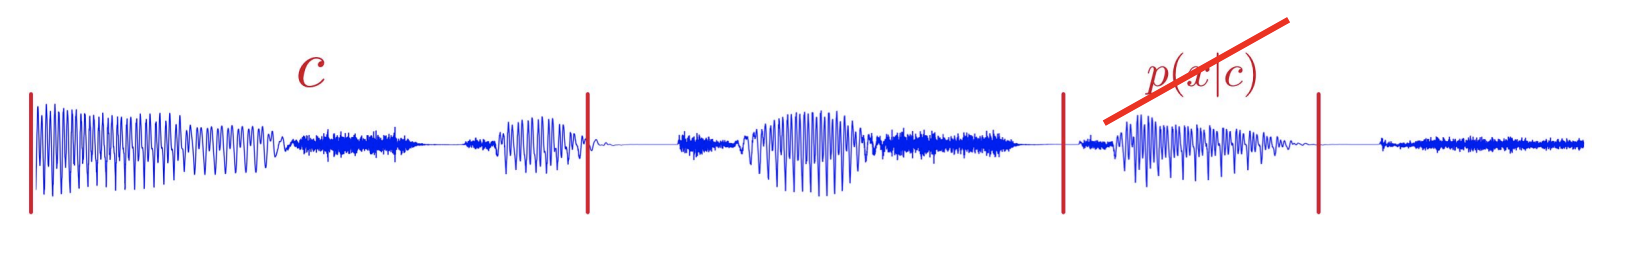
\includegraphics[width=1\linewidth,height=0.9\textheight,keepaspectratio]{images/ssl/slide_46_2_img.png}
    \end{figure}

    \framebreak

    \begin{figure}
        \centering
        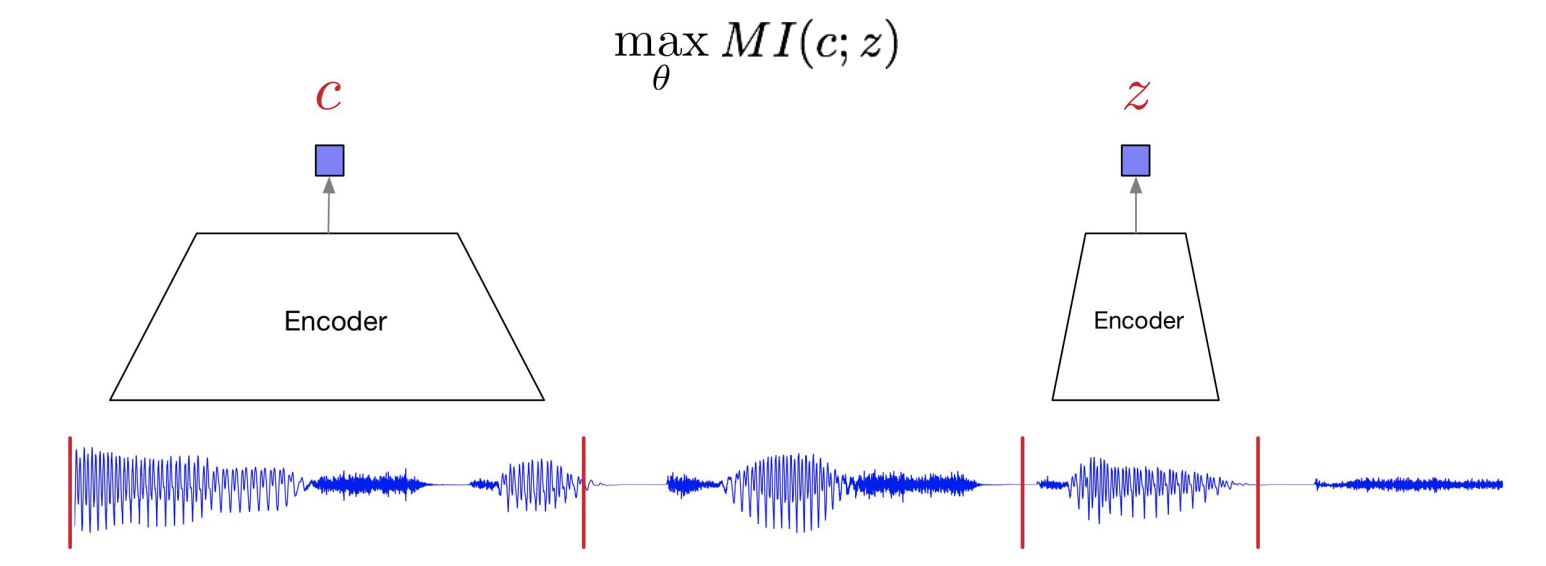
\includegraphics[width=1\linewidth,height=0.9\textheight,keepaspectratio]{images/ssl/slide_47_3_img.png}
    \end{figure}

    \framebreak

    \begin{figure}
        \centering
        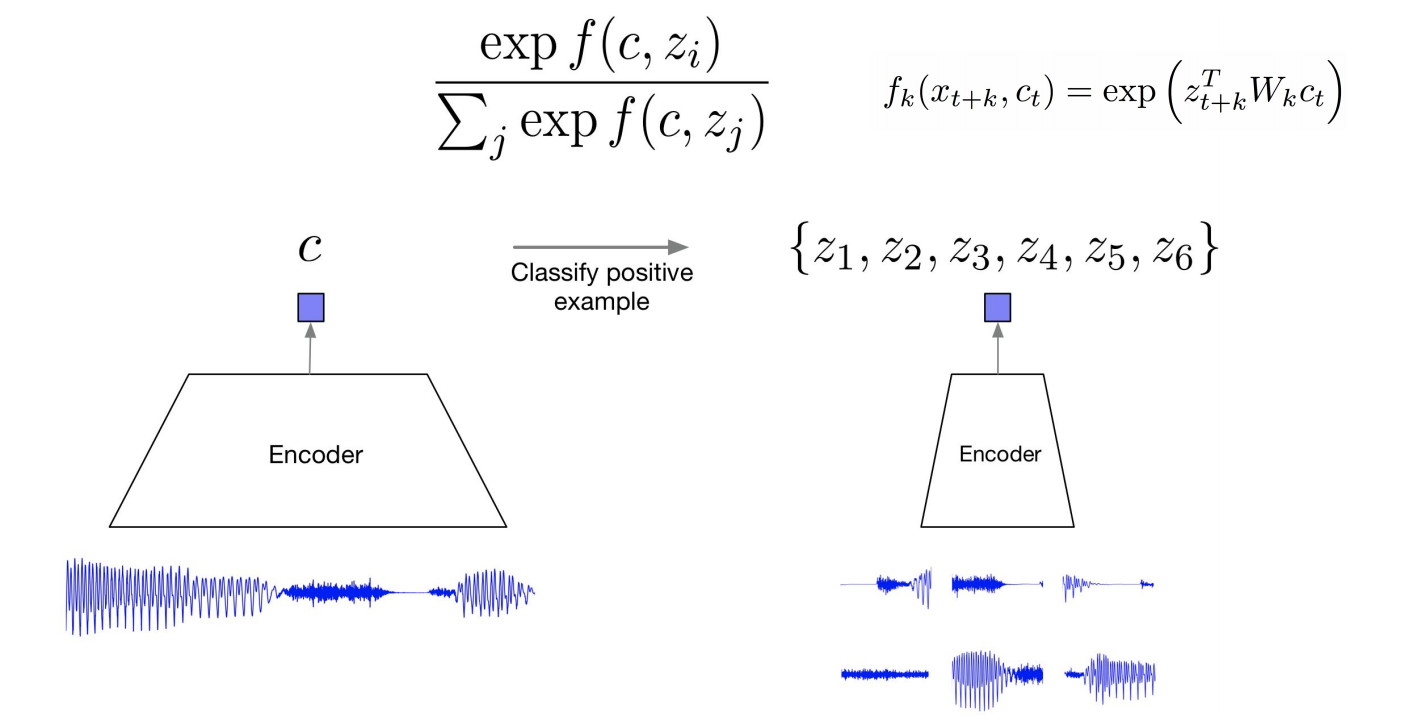
\includegraphics[width=1\linewidth,height=0.9\textheight,keepaspectratio]{images/ssl/slide_48_4_img.png}
    \end{figure}

    \framebreak

    \begin{figure}
        \centering
        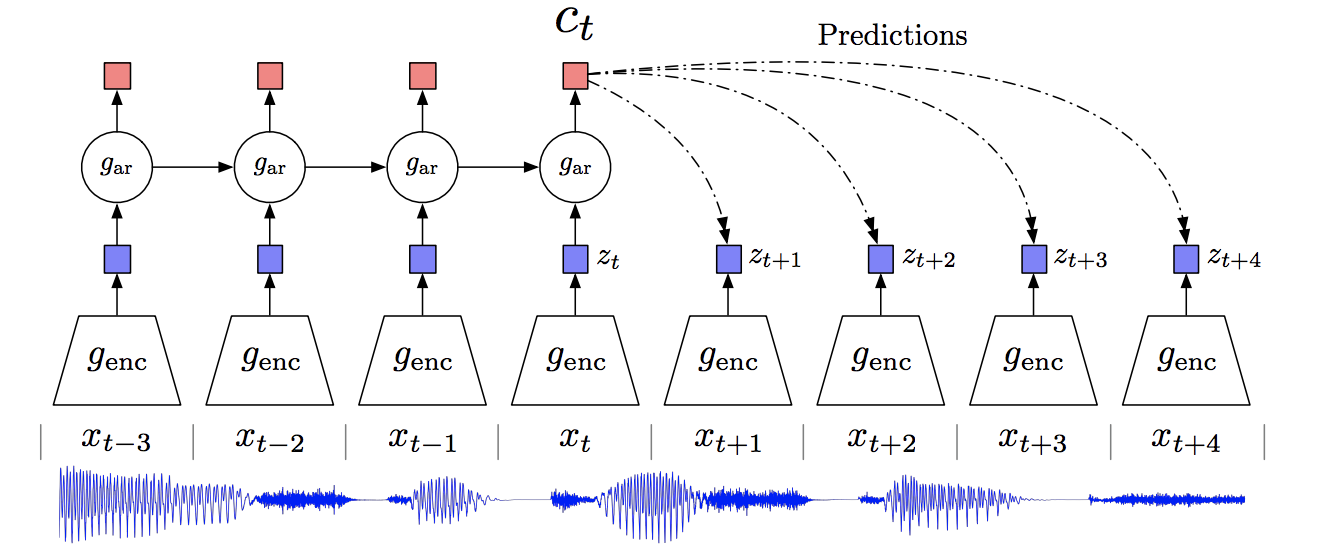
\includegraphics[width=1\linewidth,height=0.9\textheight,keepaspectratio]{images/ssl/slide_49_1_img.png}
    \end{figure}

    \framebreak

    \begin{figure}
        \centering
        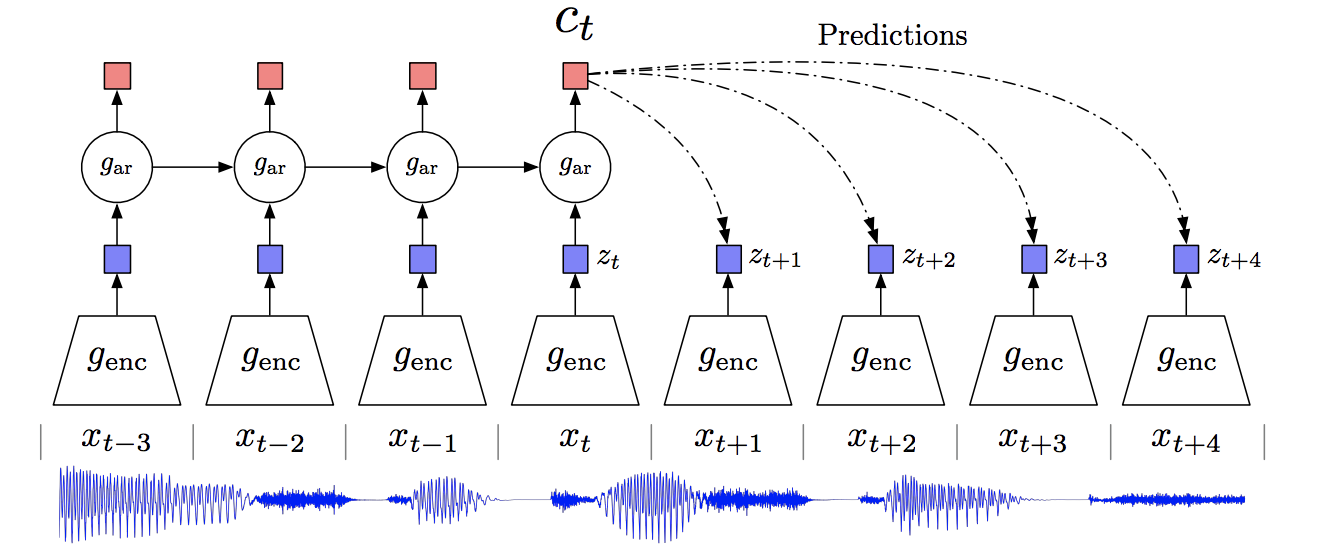
\includegraphics[width=1\linewidth,height=0.5\textheight,keepaspectratio]{images/ssl/slide_50_2_img.png}
    \end{figure}

    \begin{figure}
        \centering
        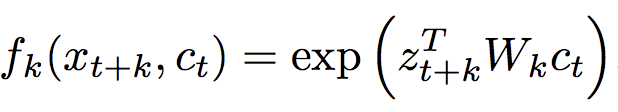
\includegraphics[width=0.5\linewidth,height=0.3\textheight,keepaspectratio]{images/ssl/slide_50_3_img.png}
    \end{figure}

    \begin{figure}
        \centering
        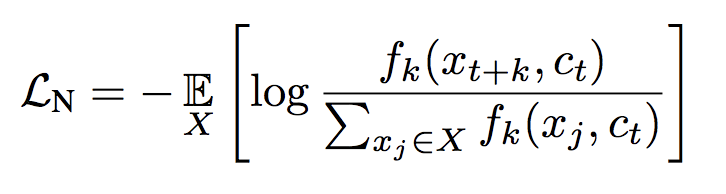
\includegraphics[width=0.5\linewidth,height=0.3\textheight,keepaspectratio]{images/ssl/slide_50_1_img.png}
    \end{figure}

    \framebreak

    \textbf{Key Points about CPC}:
    \begin{itemize}
        \item CPC learns representations by maximizing mutual information between context and future latent representations.
        \item It is widely used in audio, vision, and language domains for self-supervised pretraining.
        \item The contrastive loss enables learning without explicit labels, relying on the structure of the data itself.
    \end{itemize}
\end{frame}

\begin{frame}[allowframebreaks]{CPC: Speech}
    \begin{columns}
        \column{0.5\textwidth}
        \begin{figure}
            \centering
            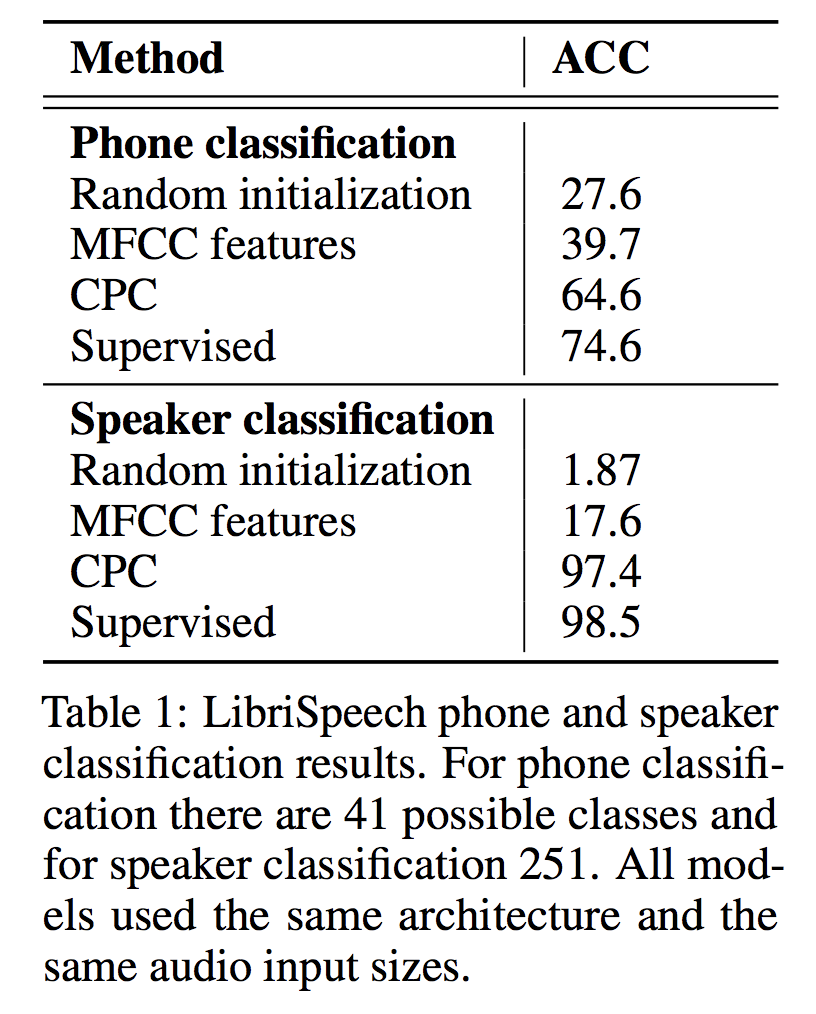
\includegraphics[width=1\linewidth,height=0.9\textheight,keepaspectratio]{images/ssl/slide_52_1_img.png}
        \end{figure}

        \column{0.5\textwidth}
        \begin{figure}
            \centering
            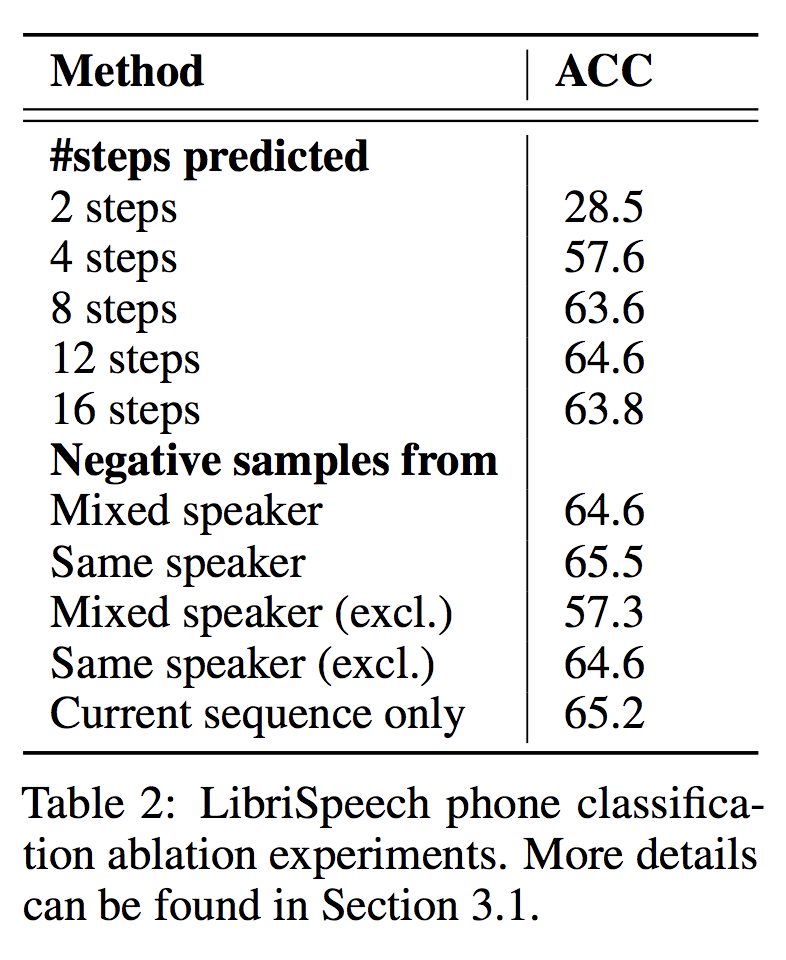
\includegraphics[width=1\linewidth,height=0.9\textheight,keepaspectratio]{images/ssl/slide_52_2_img.png}
        \end{figure}
    \end{columns}
\end{frame}

\begin{frame}[allowframebreaks]{CPC: ImageNet}
    \begin{figure}
        \centering
        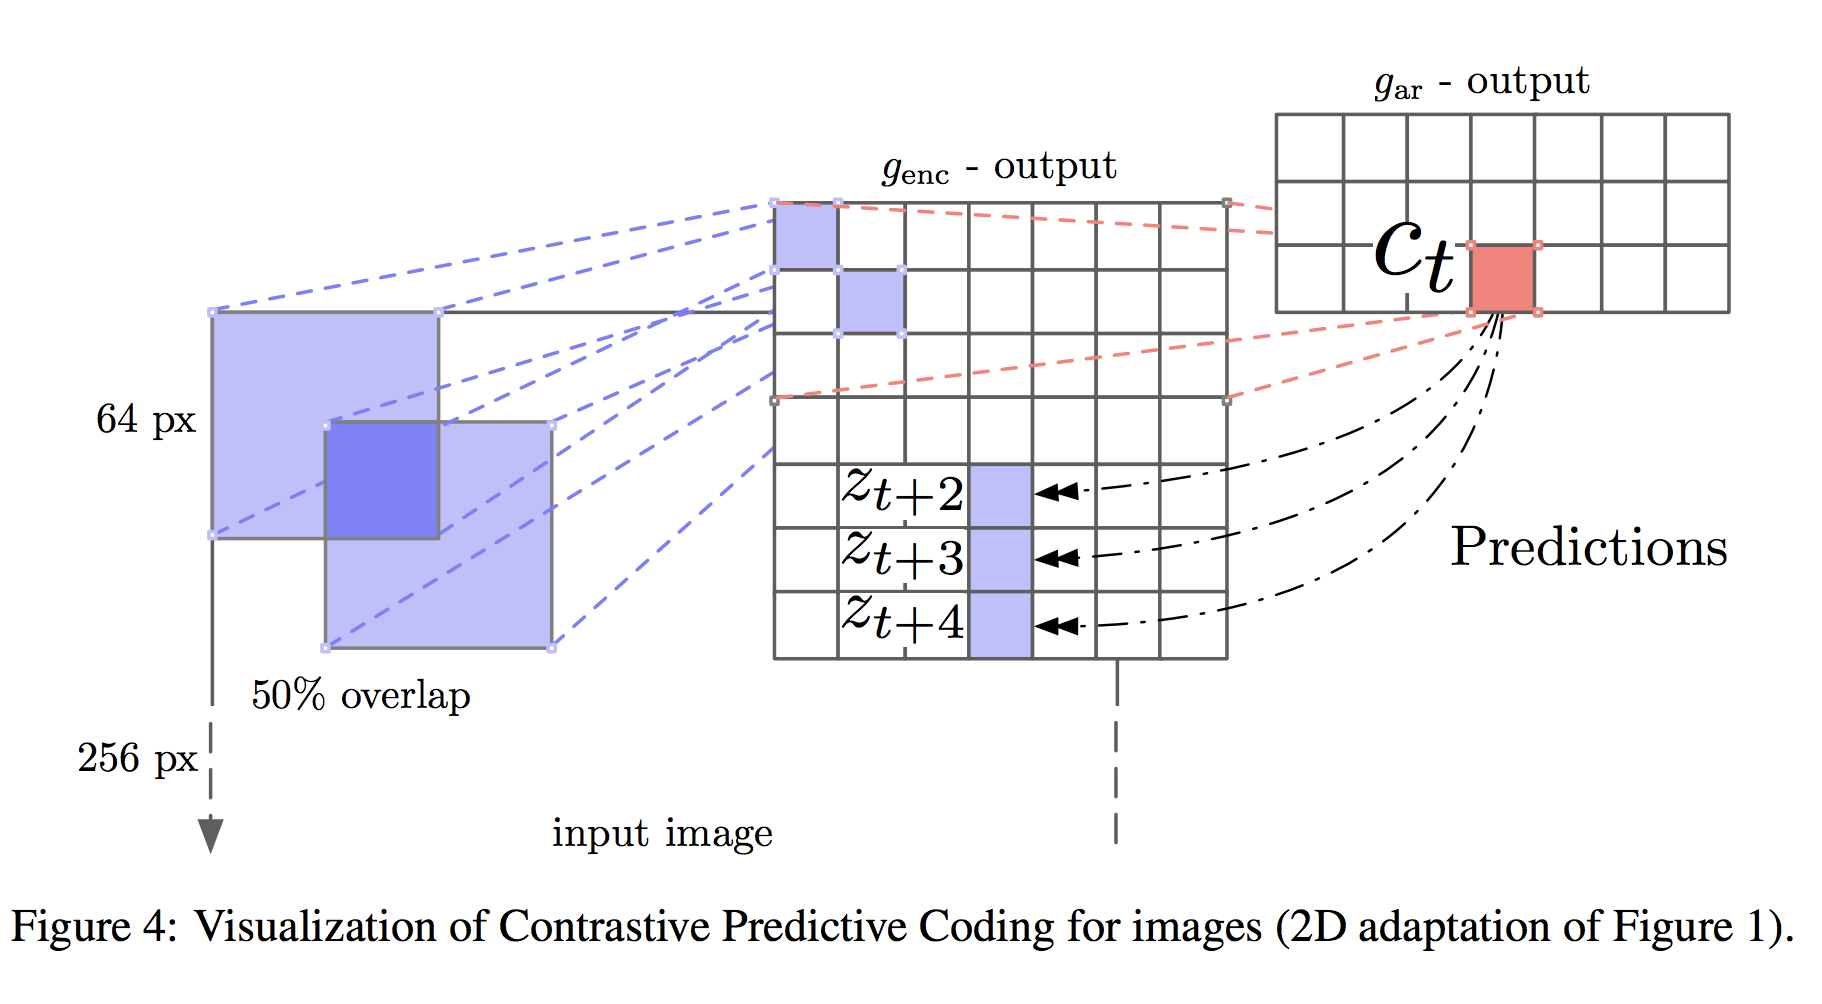
\includegraphics[width=1\linewidth,height=0.9\textheight,keepaspectratio]{images/ssl/slide_53_1_img.png}
    \end{figure}

    \framebreak

    \begin{columns}
        \column{0.5\textwidth}
        \begin{figure}
            \centering
            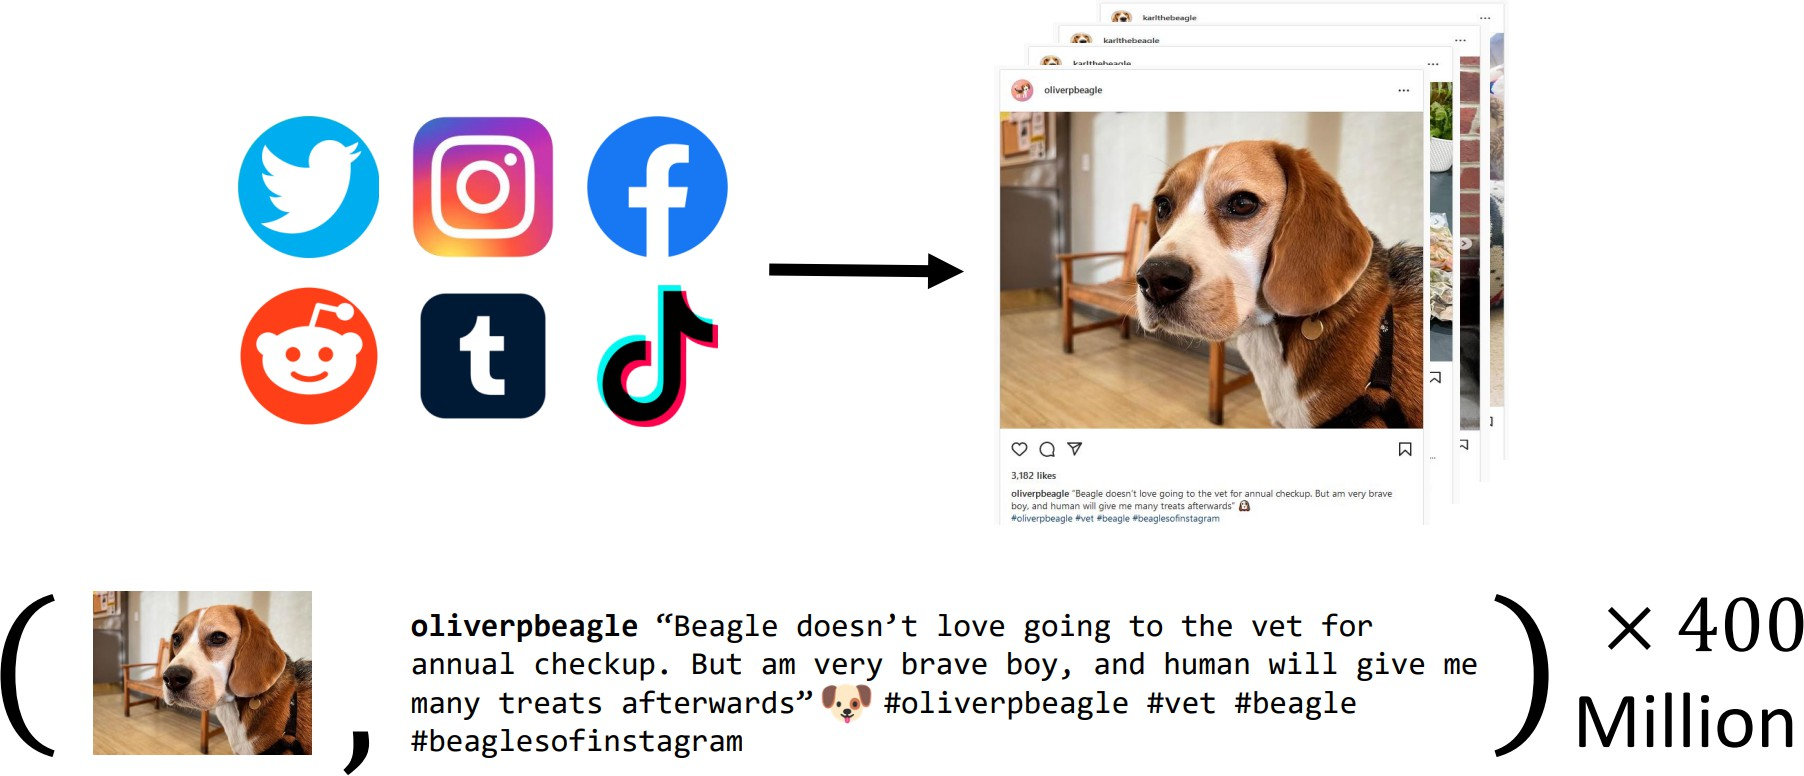
\includegraphics[width=1\linewidth,height=0.9\textheight,keepaspectratio]{images/ssl/slide_54_1_img.png}
        \end{figure}

        \column{0.5\textwidth}
        \begin{figure}
            \centering
            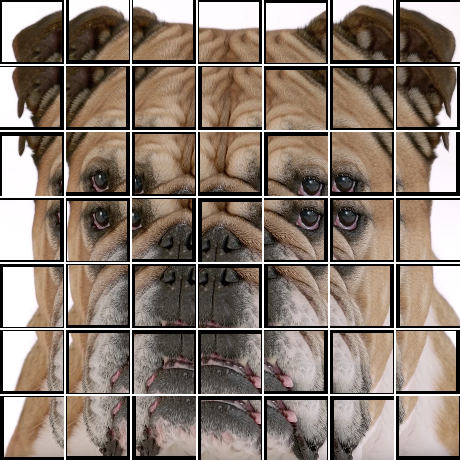
\includegraphics[width=1\linewidth,height=0.9\textheight,keepaspectratio]{images/ssl/slide_54_2_img.png}
        \end{figure}
    \end{columns}

    \framebreak

    \begin{figure}
        \centering
        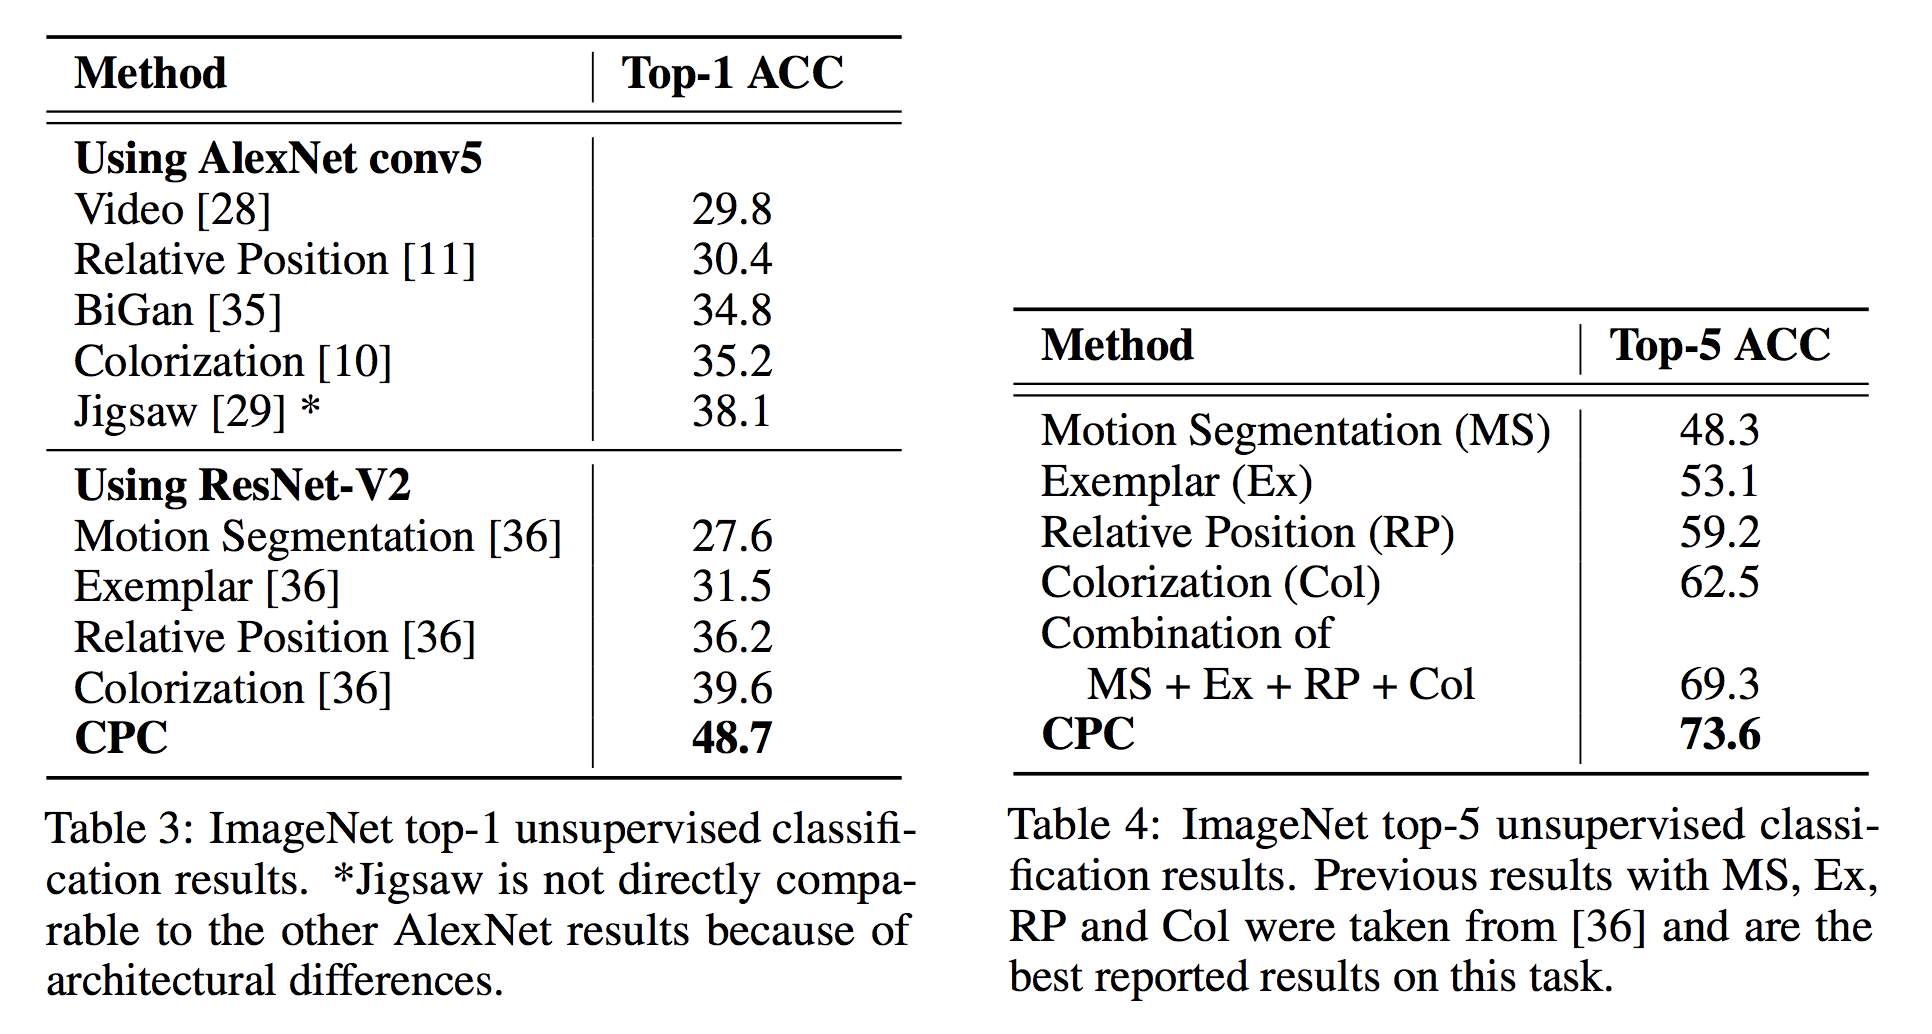
\includegraphics[width=1\linewidth,height=0.9\textheight,keepaspectratio]{images/ssl/slide_55_1_img.png}
    \end{figure}

    \framebreak

    \begin{figure}
        \centering
        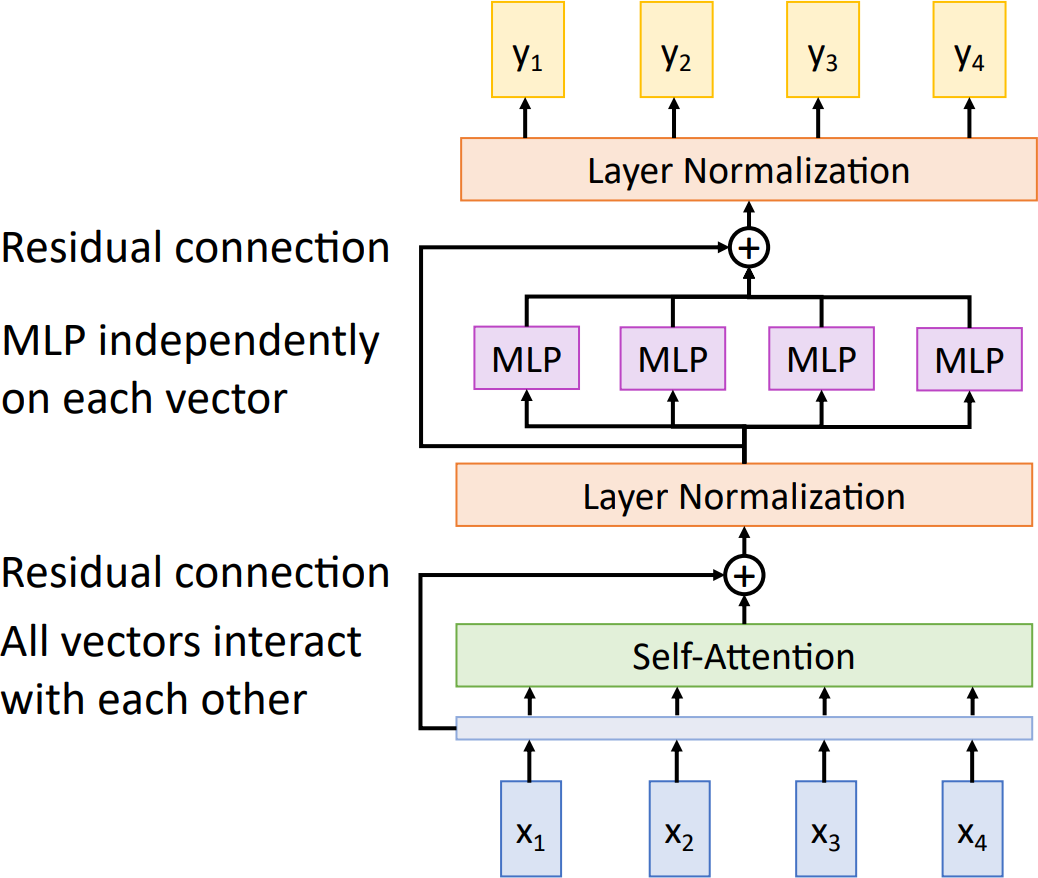
\includegraphics[width=1\linewidth,height=0.9\textheight,keepaspectratio]{images/ssl/slide_56_1_img.png}
    \end{figure}
\end{frame}


\begin{frame}[allowframebreaks]{CPC: Natural Language Processing}
    \begin{figure}
        \centering
        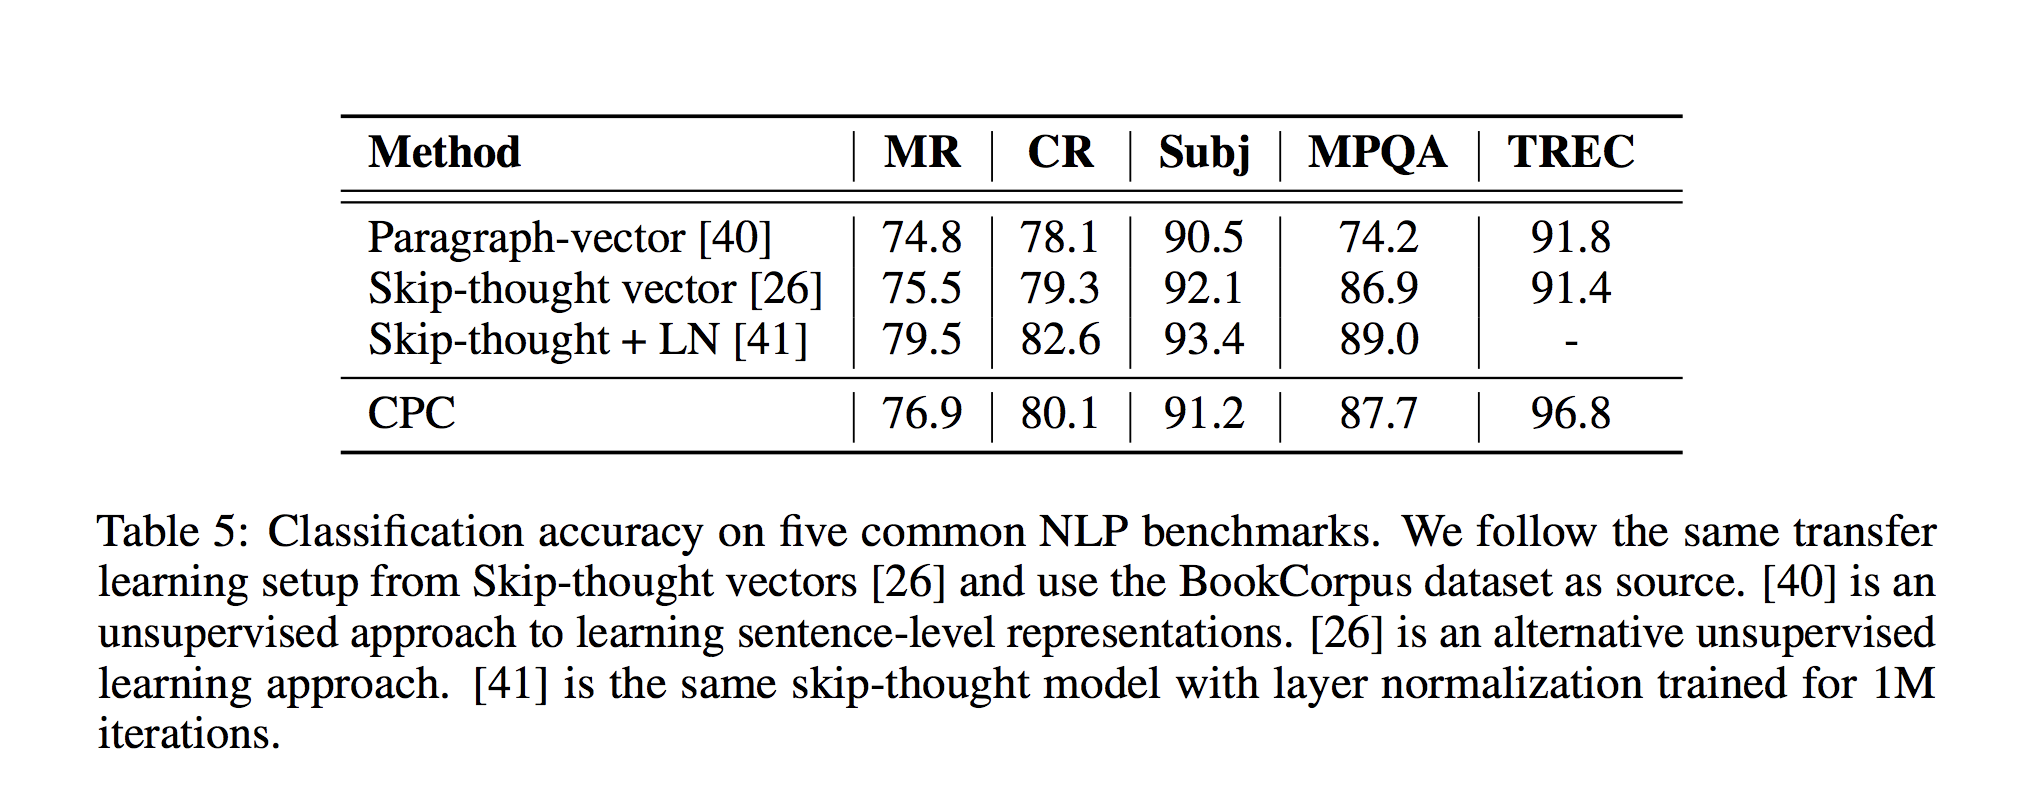
\includegraphics[width=1\linewidth,height=0.9\textheight,keepaspectratio]{images/ssl/slide_57_1_img.png}
    \end{figure}
\end{frame}


\begin{frame}[allowframebreaks]{CPC: Reinforcement Learning}
    \begin{figure}
        \centering
        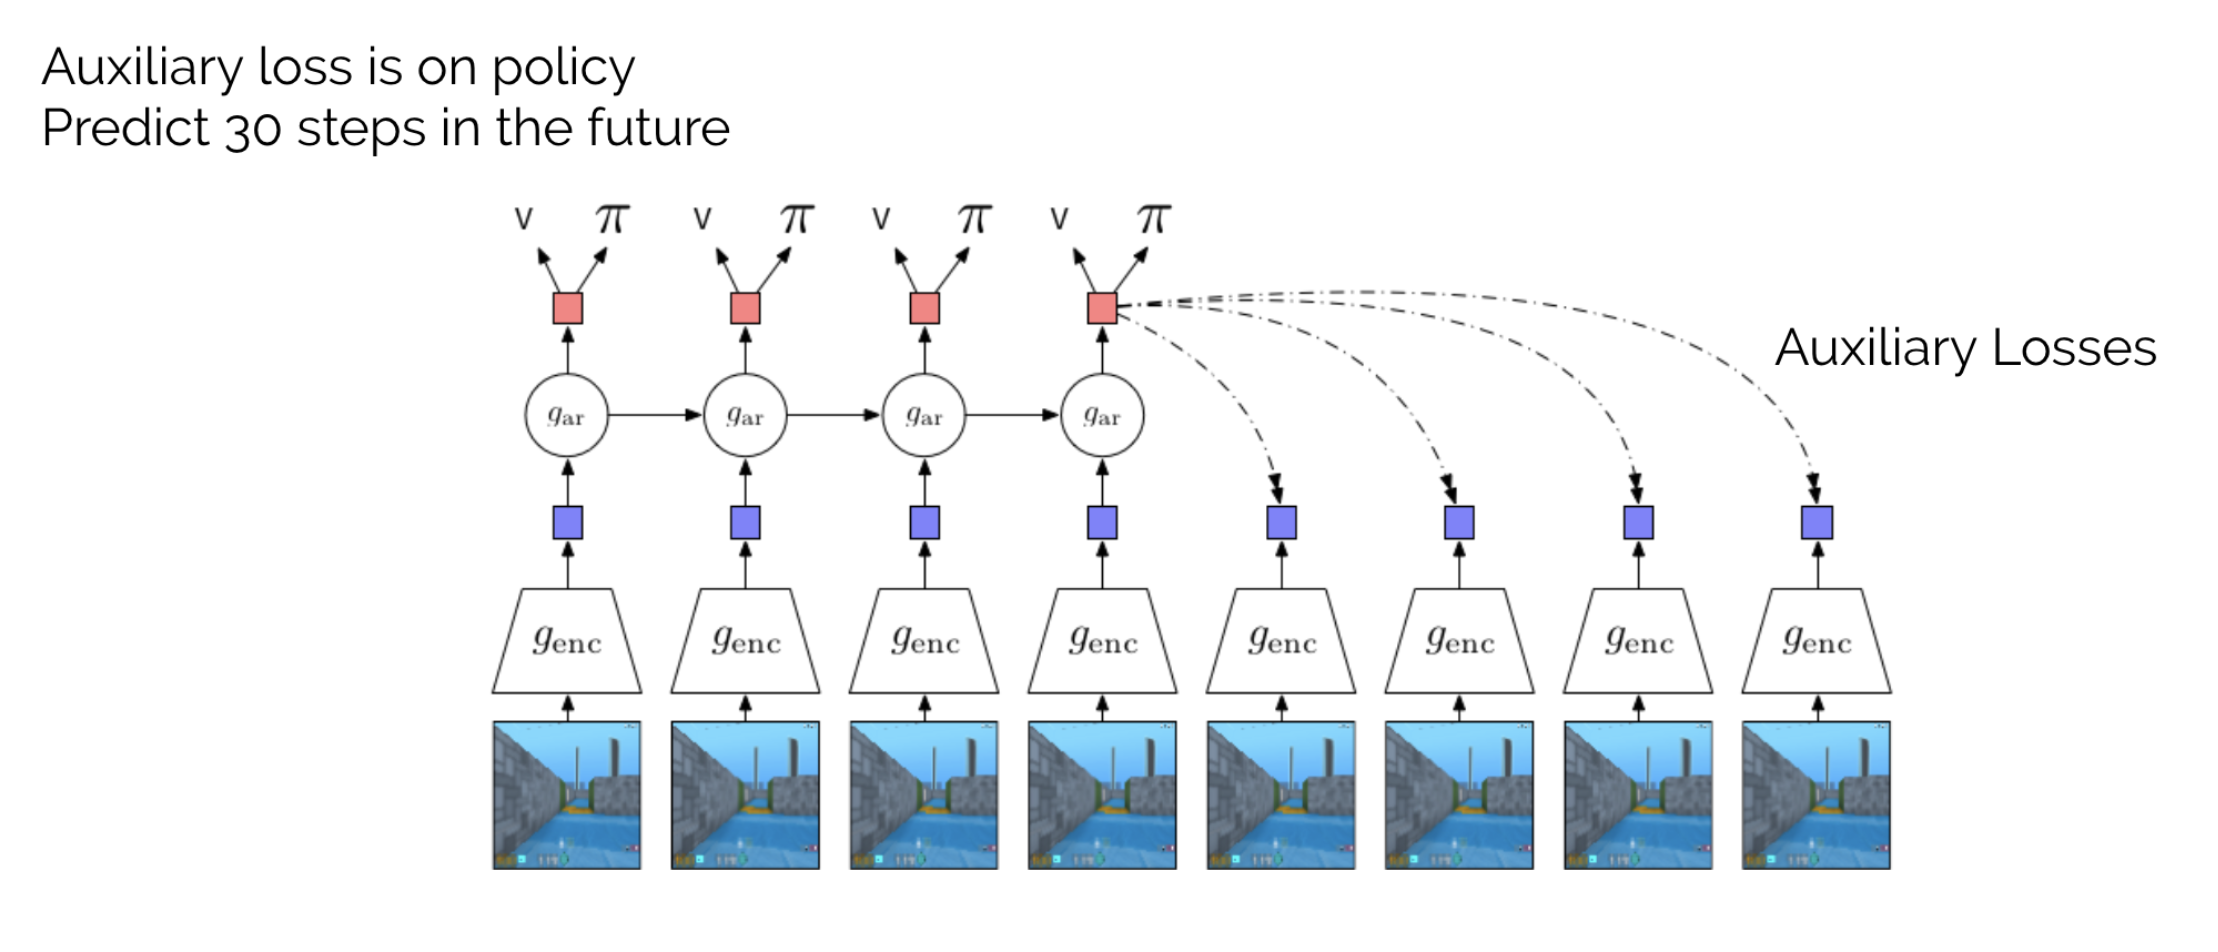
\includegraphics[width=1\linewidth,height=0.9\textheight,keepaspectratio]{images/ssl/slide_58_1_img.png}
    \end{figure}
\end{frame}


\begin{frame}[allowframebreaks]{CPCv2: Large Scale CPC on ImageNet}
    \begin{figure}
        \centering
        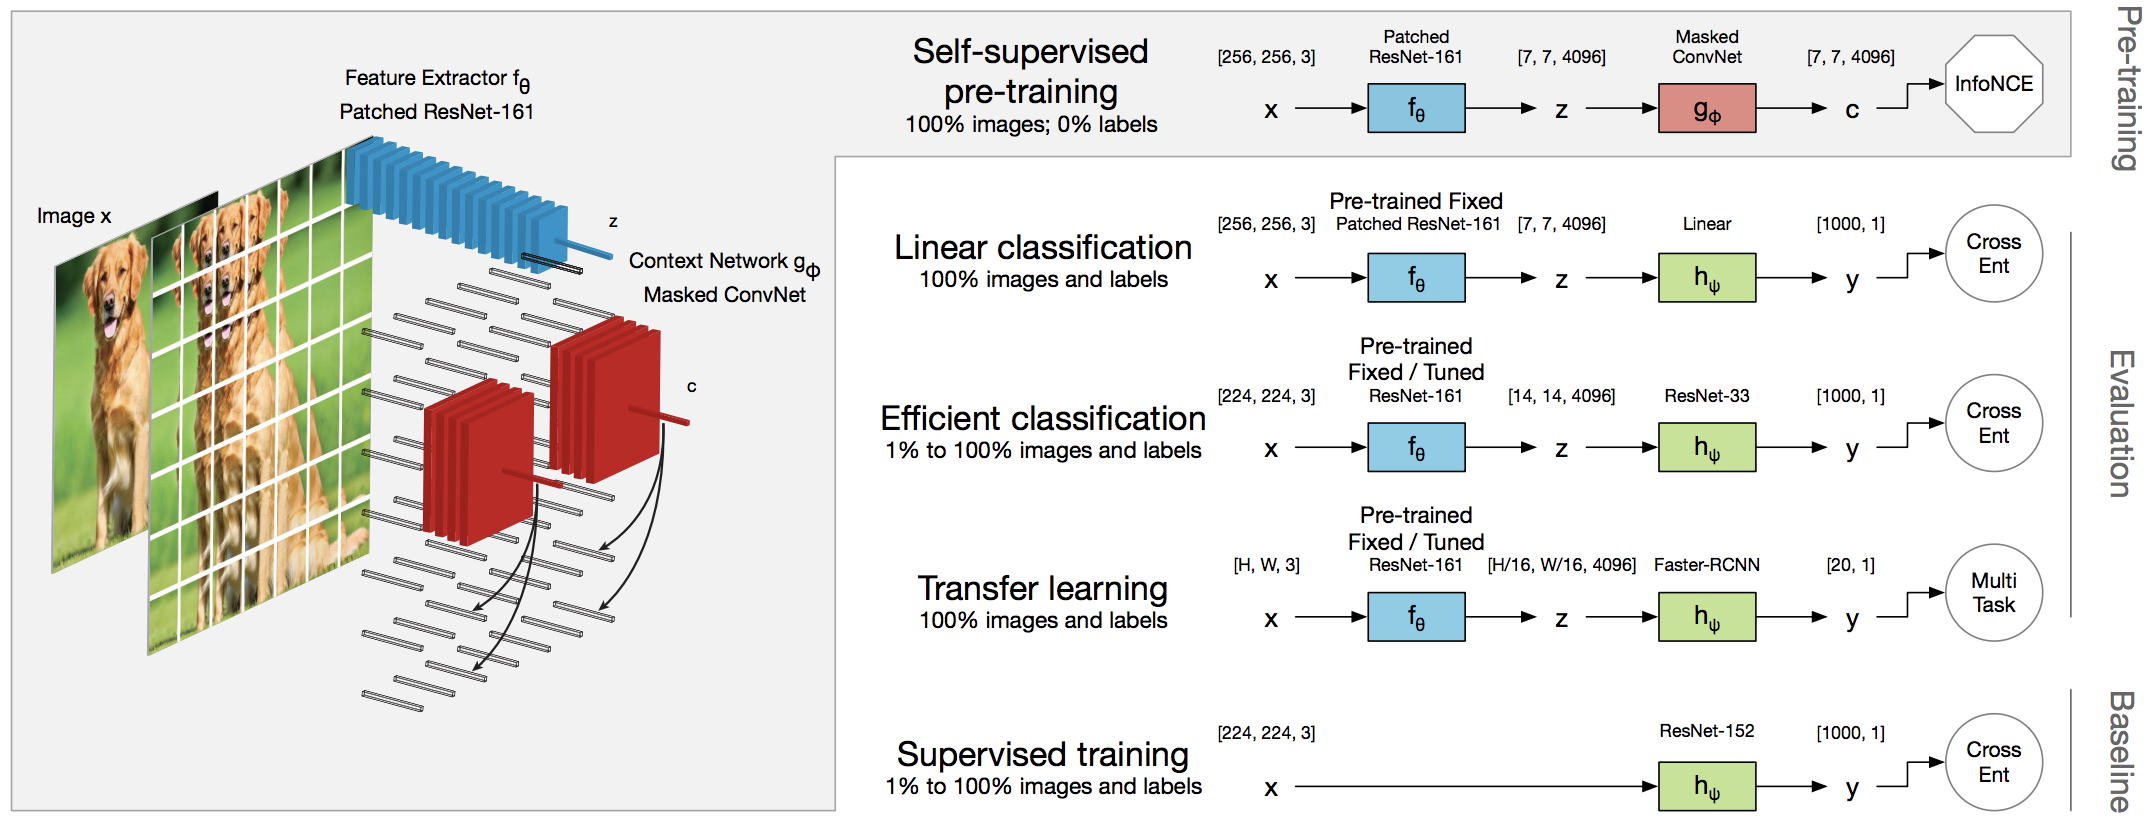
\includegraphics[width=1\linewidth,height=0.9\textheight,keepaspectratio]{images/ssl/slide_59_1_img.png}
    \end{figure}
\end{frame}

\begin{frame}[allowframebreaks]{CPCv2: Linear Classification}
    \begin{figure}
        \centering
        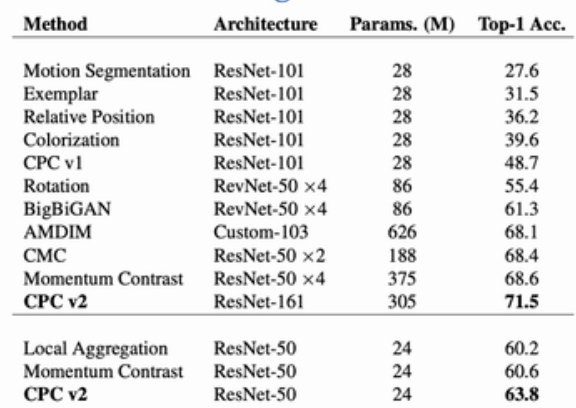
\includegraphics[width=1\linewidth,height=0.9\textheight,keepaspectratio]{images/ssl/slide_60_1_img.png}
    \end{figure}
\end{frame}


\begin{frame}[allowframebreaks]{CPCv2: Data-Efficient Image Recognition}
    \begin{figure}
        \centering
        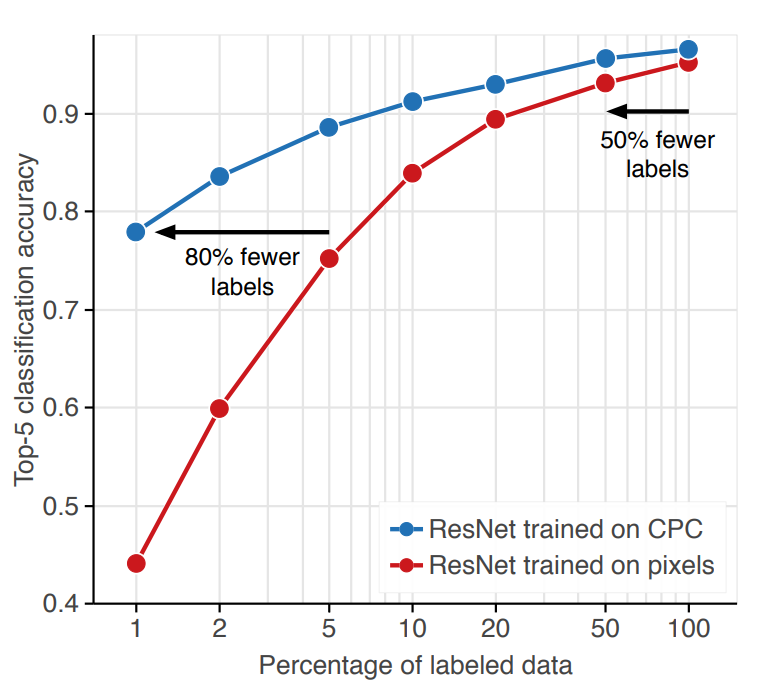
\includegraphics[width=1\linewidth,height=0.9\textheight,keepaspectratio]{images/ssl/slide_61_1_img.png}
    \end{figure}
\end{frame}


\begin{frame}[allowframebreaks]{CPCv2: Data-Efficient Supervised Learning}
    \begin{figure}
        \centering
        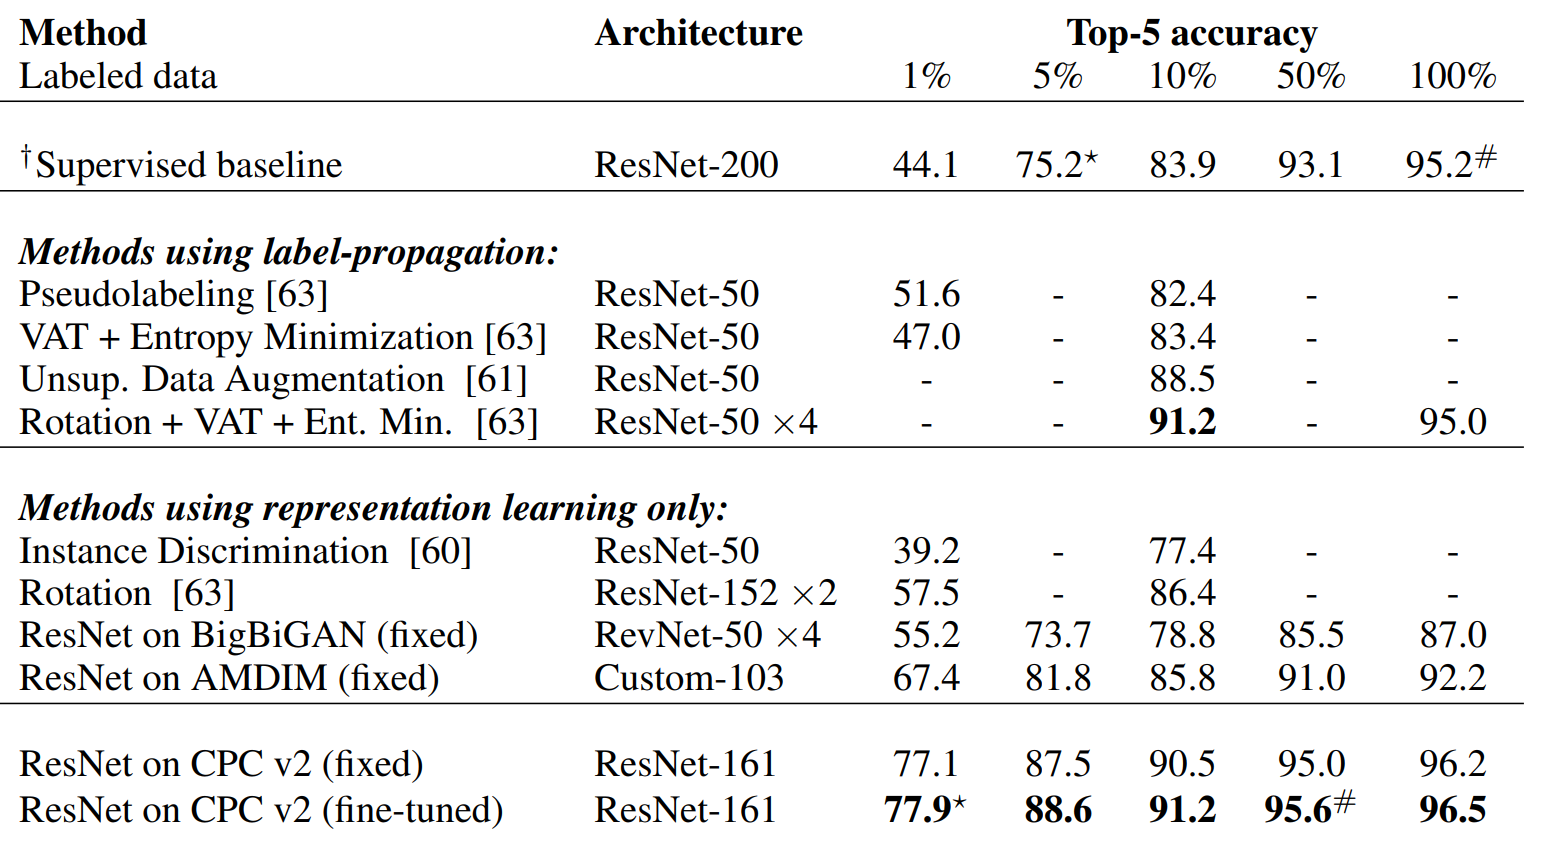
\includegraphics[width=1\linewidth,height=0.9\textheight,keepaspectratio]{images/ssl/slide_62_1_img.png}
    \end{figure}
\end{frame}